\documentclass[usenatbib]{mn2e} 
\usepackage{amsmath} 
\usepackage{amssymb} 
\usepackage{graphics}
\usepackage{graphicx}
\usepackage{epsfig} 
\usepackage{float} 
\def\be{\begin{equation}}
\def\ee{\end{equation}}
\def\ba{\begin{eqnarray}}
\def\ea{\end{eqnarray}}

% To highlight comments 
\usepackage{color}
\definecolor{red}{rgb}{1,0.0,0.0}
\newcommand{\red}{\color{red}}
\definecolor{blue}{rgb}{0.1,0.3,0.9}
\newcommand{\blue}{\color{blue}}

\usepackage[normalem]{ulem}
\definecolor{darkgreen}{rgb}{0.0,0.5,0.0}
\newcommand{\SRK}[1]{\textcolor{darkgreen}{\bf SRK: \textit{#1}}}
\newcommand{\SRKED}[1]{\textcolor{darkgreen}{\bf #1}}

\newcommand{\LCDM}{$\Lambda$CDM~}
\newcommand{\beq}{\begin{eqnarray}}  
\newcommand{\eeq}{\end{eqnarray}}  
\newcommand{\zz}{$z\sim 3$} 
\newcommand{\apj}{ApJ}  
\newcommand{\apjs}{ApJS}  
\newcommand{\apjl}{ApJL}  
\newcommand{\aj}{AJ}  
\newcommand{\mnras}{MNRAS}  
\newcommand{\mnrassub}{MNRAS accepted}  
\newcommand{\aap}{A\&A}  
\newcommand{\aaps}{A\&AS}  
\newcommand{\araa}{ARA\&A}  
\newcommand{\nat}{Nature}  
\newcommand{\physrep}{PhR}
\newcommand{\pasp}{PASP}    
\newcommand{\pasj}{PASJ}    
\newcommand{\avg}[1]{\langle{#1}\rangle}  
\newcommand{\ly}{{\ifmmode{{\rm Ly}\alpha}\else{Ly$\alpha$}\fi}}
\newcommand{\hMpc}{{\ifmmode{h^{-1}{\rm Mpc}}\else{$h^{-1}$Mpc }\fi}}  
\newcommand{\hGpc}{{\ifmmode{h^{-1}{\rm Gpc}}\else{$h^{-1}$Gpc }\fi}}  
\newcommand{\hmpc}{{\ifmmode{h^{-1}{\rm Mpc}}\else{$h^{-1}$Mpc }\fi}}  
\newcommand{\hkpc}{{\ifmmode{h^{-1}{\rm kpc}}\else{$h^{-1}$kpc }\fi}}  
\newcommand{\hMsun}{{\ifmmode{h^{-1}{\rm {M_{\odot}}}}\else{$h^{-1}{\rm{M_{\odot}}}$}\fi}}  
\newcommand{\hmsun}{{\ifmmode{h^{-1}{\rm {M_{\odot}}}}\else{$h^{-1}{\rm{M_{\odot}}}$}\fi}}  
\newcommand{\Msun}{{\ifmmode{{\rm {M_{\odot}}}}\else{${\rm{M_{\odot}}}$}\fi}}  
\newcommand{\msun}{{\ifmmode{{\rm {M_{\odot}}}}\else{${\rm{M_{\odot}}}$}\fi}}  
\newcommand{\lya}{{Lyman$\alpha$~}}
\newcommand{\clara}{{\texttt{CLARA}}~}
\newcommand{\rand}{{\ifmmode{{\mathcal{R}}}\else{${\mathcal{R}}$ }\fi}}  
\newcommand{\hs}{{\hspace{1mm}}}  

% definition to produce a "less than or similar to" symbol
\def\lsim{~\rlap{$<$}{\lower 1.0ex\hbox{$\sim$}}}

% definition to produce a "greater than or similar to" symbol
\def\gsim{~\rlap{$>$}{\lower 1.0ex\hbox{$\sim$}}}

\begin{document}

\title[Rotation in the Lyman-$\alpha$ line]{Effects of bulk gas rotation on
  the emergent Lyman-$\alpha$ line in distant galaxies}
\author[N. Garavito and J.E. Forero-Romero]{
\parbox[t]{\textwidth}{\raggedright 
  Nicolas Garavito-Camargo.$^{1}$ 
  Jaime E. Forero-Romero$^{2}$ 
}
\vspace*{6pt}\\
$^{1}$Uni A
$^{2}$Uni B
}
\maketitle

\begin{abstract}

\end{abstract}
\begin{keywords}
galaxies: high-redshift - galaxies: star formation - line: formation
\end{keywords}


\section{Introduction}
\label{sec:intro}

Due to the resonant nature of the lyman alpha line, gas kinematics
play an important role in the shape of this line. In particular we
study the case in which this gas is spherically symmetric and its
rotating.


\section{Implementation of Bulk Gas Rotation}
\label{sec:implementation}

We implement into CLARA the simplest model whereby a sphere rotates
with homogeneous angular velocity. We define a cartesian coordinate
system with its origin at the center of the sphere and the rotation
axis to be the $z$-axis, the components in the bulk velocity field, $\vec{v}
= v_{x}\hat{i} + v_{y}\hat{j} + v_{z}\hat{k}$. in the gas can be written as 
 
%In cartesian coordinates the rotational velocity around de the z-axys
%is defined by:

\begin{subequations}
\begin{align}
    v_{x}=-\dfrac{y}{R}V_{\rm max}, \label{subeq1}\\
    v_{y}=\dfrac{x}{R}V_{\rm max}, \label{subeq2}\\
    v_{z}=0, \label{subeq3}
\end{align}
\end{subequations}

%Where $x$ and $y$ define de position of the gas atoms and dust
%particles. 
%The minus sign in the x-component of the velocity is due to
%the direction of rotation, in this case we assume that as seeing from
%the top,the rotation is anticlockwise.
where $R$ is the radius of the sphere and $V_{\rm max}$ is the linear
velocity at the sphere's surface. The minus sign in the x-component of the velocity is due to
the direction of rotation, in this case we assume that the angular
velocity vector goes in the $\hat{k}$ direction.


\section{Grid of Simulated Models}
\label{sec:models}

%We propose several models which include differents rotational
%velocities and optical depths. We also take into account the dust
%within the gas and two differents initial distributions of the
%photons, central and homogeneous. At the end we study 48 models, those
%are resumed in Table[1]\\ 

We compute the emergent Lyman-$\alpha$ line for several models with
differents values for the maximal rotational velocity, hydrogend optical
depth, dust optical depth and initial distributions of the photons
with respect to the gas. There are in total 60 models with the input
parameters summarized in Table  \ref{table:models}. 

% JF: digo que son 60 modelos porque estoy incluyendo los de velocidad cero.

%We later study this models taking into account the posititon of the
%observer respect to the axis of rotation of the cloud. 

Additionaly in the postprocessing process we will take into account
different observer positions with respect to the cloud rotation
axis.


\begin{table}
\begin{center}
\begin{tabular}{ccc}\hline
Velocity (km s$^{-1}$) & $V_{\rm max}$&$0,\ 50,\ 100,\ 200,\ 300$\\
Hydrogen Optical Depth & $\tau_{H} $ & $10^{5},\ 10^{6},\ 10^{7}$\\
Dust Optical Depth & $\tau_{A}$ & XXX \\
Photons Distributions & & Central, Homogeneous\\
\hline
\end{tabular}
\caption{
Values for the varying input parameters in CLARA. Taking into account
all the possible combinations for these models
} 
\label{table:models}
\end{center}
\end{table}



\begin{figure*}
  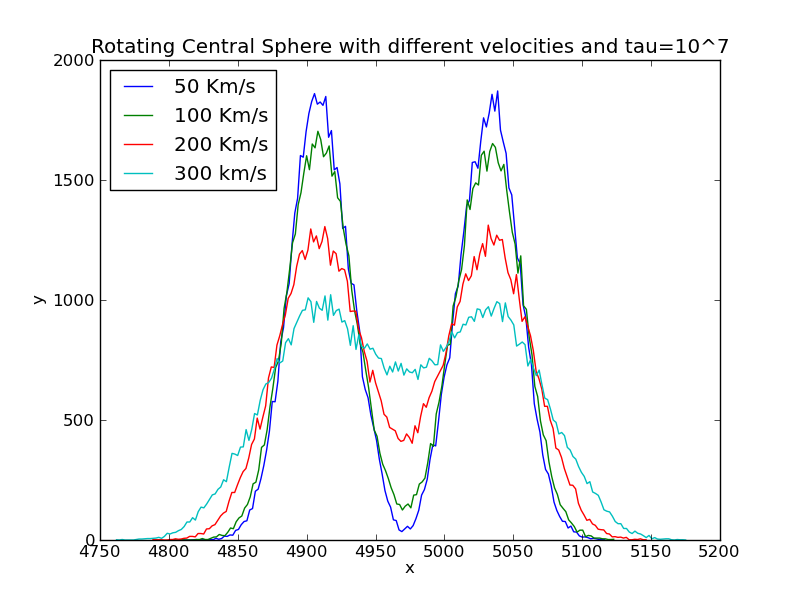
\includegraphics[width=0.45\textwidth]{7tDifSpeedsZ.png}
  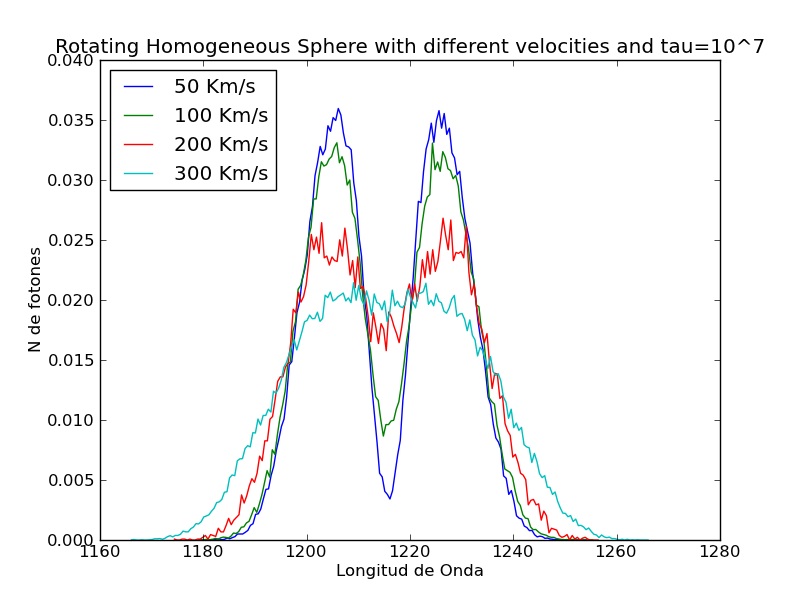
\includegraphics[width=0.45\textwidth]{7tHOMDifSpeeds1.png}
  \label{fig:HOMandCentral}\caption{Shape of the lyman alpha line for
    differents velocities. The left panel show the central
    distribution while the right panel show the homogeneous
    distribution.}
\end{figure*}


Now if we take into account the position of the observer and compute
this for differents angles of observation $\theta$ the outcoming
spectra is modified as is shown in Figure~\ref{DifferentObservers}. The main feature here is that as the angle increases the line height decreases. It means that a observer in the poles will observe a higher double peak than a
observer in the ecuator. We will understand this in more detail when
we present the results of the scape fraction in section~\ref{sec:EF}.      

\begin{figure}
\begin{center}
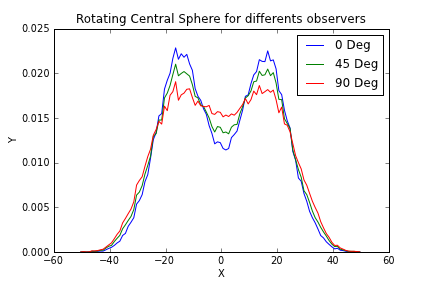
\includegraphics[scale=0.45]{Observers.png}
\end{center}
\caption{Spectra for different observers. Model:$V=300km/s$, Optical
  Depth $\tau=10^{7}$ and Central Distribution without dust.} 
  \label{DifferentObservers}
\end{figure}

%describir los modelos, poner las ecuaciones de la velocidad de
%rotacion, %poner las graficas para un modelo dado poner el efecto de
%la rotación (poner %uno con velocidad cero) y del observador. 



\section{Results}
\label{sec:Results}

%Ver correo de Jaime y tratar de explicar a que se deben estos efectos.


In the previous section we describe the models that we use to study the
effect of rotation in the Lyman alpha line for this we saw the outcoming specrtums including rotation. Now we show the main results that we
obtain, in particual we pay spetial attention to the position of the
maximums, the width of the line and the escape fraction in function of
the rotational velocity and the angle of observation $\theta$.  

In Figure~\ref{fig:HOMandCentral} the effect that rotation have in the spectra is shown,
for both distributions central (Left) and homogeneous (right). This is
a general case in the sense that is independent of the position of an
external observer.  

\subsection{Maxima Positions}
\label{sec:MP}

\begin{figure}
    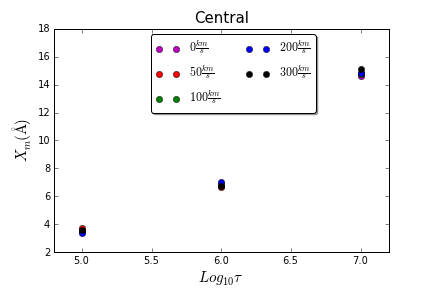
\includegraphics[width=0.45\textwidth]{maximumvsODDifSpeedsCentral.png}
    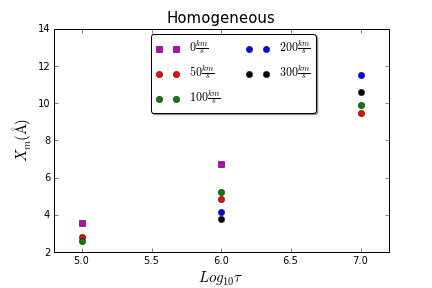
\includegraphics[width=0.45\textwidth]{maximumvsODDifSpeedsHOM.png}
  \label{figure:maximavsOD}\caption{Position of the maxima in the outgoing spectra for differents Optical Depths, (up)Central Distriution, (Down) Homogeneous Distribution.}
\end{figure}


\begin{figure}
    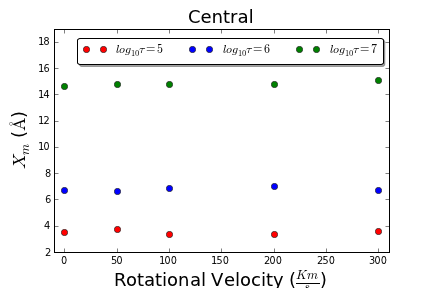
\includegraphics[width=0.45\textwidth]{maximumvsvelocitiesDifODCentral.png}
    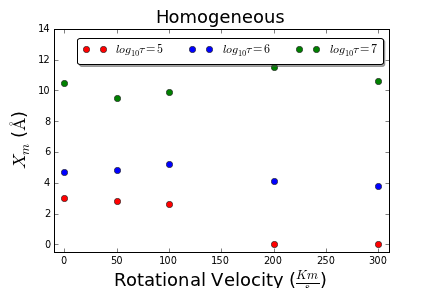
\includegraphics[width=0.45\textwidth]{maximumvsvelocitiesDifODHOM.png}
  \label{figure:maximumsvsvelocities}\caption{Position of the maxima in the outgoing spectra for differents Rotational velocities, (up)Central Distriution, (Down) Homogeneous Distribution.}
\end{figure}

The maximums position gives information about the wave lenght of the
mayority of the outcoming photons after they interact with the gas, in
addition as a photon have more scatterings its wave lenght would be
larger than the initial which is $1216$ {\AA}. 
As we can see in Figure ~\ref{figure:maximumsvsvelocities} the position of the maximums does not change with rotational velocity for the central dsitribution. On the other hand for the homogeneous distriution the maxima position $X_{m}$ change for $Log_{10}\tau=5$, this is because at higher rotational velocities photons escape with less scatterings, for $v=100\dfrac{km}{s}$ the majority of the photons still escape with scatterings but for $v=200\dfrac{km}{s}$ the number of photons that escape with a few or any scatterings is higher, this is why the maxima change to the center of the spectra.\\

If we now study the effect of the optical depth $\tau$ in the maxima position $X_{m}$ Figure~\ref{figure:maximavsOD}, we found that as the optical depth increase (include reference of previous articles) the maxima position increase and this is a well known result, but when rotation is included the dependence is not linear.
%(think a lit bit more on this, maybe make a regression)
%explain the method to find the maxima position

\subsection{Line Width}
\label{sec:LW}

Another effect that the rotation of the gas produce is in the  width
of the lyman alpha line. The width of the line provide information of
how many photons scape with a particular wave lenght, in the
ideal case in which all the photons scape with the same wave lenght
the outcoming spectrum would be narrower. For all the models we study we
found that as the rotational velocity increase the line width
increase this is show in Fig.[4].\\ 
 

\begin{figure*}
    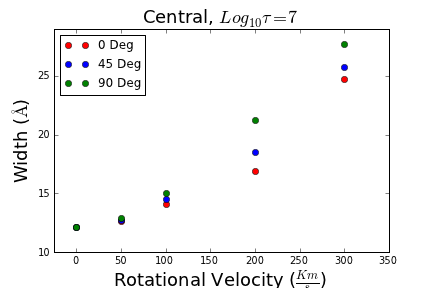
\includegraphics[width=0.45\textwidth]{Width7Central.png}
    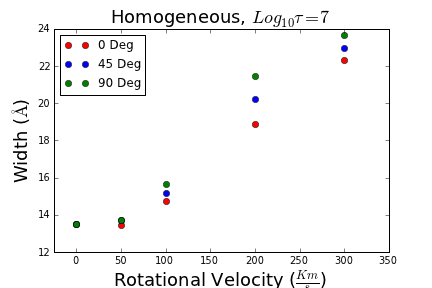
\includegraphics[width=0.45\textwidth]{Width7Homogeneous.png}
    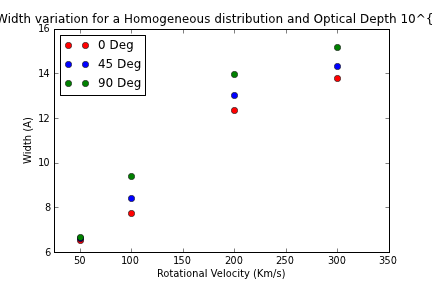
\includegraphics[width=0.45\textwidth]{Width6.png}
    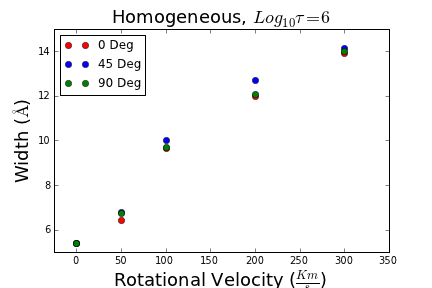
\includegraphics[width=0.45\textwidth]{Width6HOM.png}
    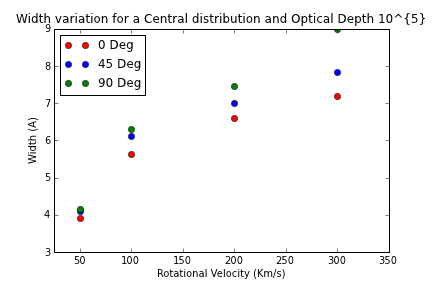
\includegraphics[width=0.45\textwidth]{Width5.png}
    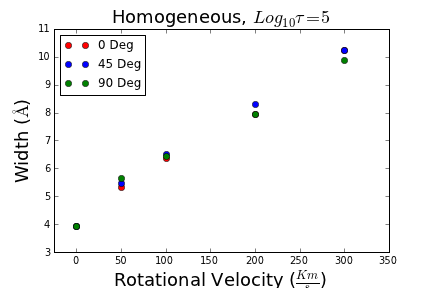
\includegraphics[width=0.45\textwidth]{Width5HOM.png}
  \label{figure:width}\caption{Width of the lyman-alpha line for all the models. }
\end{figure*}

We also found that the width for a particular model is not the same
for differents angles of observation in particular as the angle
increase the width also increase, it means that as the angle increase
the number of scatterings of the photons increasse for this reason we
see a broader line. Fig.[5]\\ 

\begin{figure}
\begin{center}
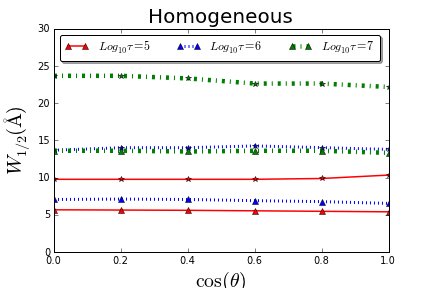
\includegraphics[width=0.45\textwidth]{WidthvsTheta.png}
\caption{Width variation in function of theta}
\end{center}
\end{figure}




\subsection{Escape Fraction}
\label{sec:EF}

The fraction of photons that escape from the cloud of gas and dust is
defined as:\\ 

\begin{equation}
F_{e}=\dfrac{\Sigma_{NI} \vec{k}\cdot \vec{o}}{\Sigma_{NF}\vec{k}\cdot \vec{o}}
\end{equation}

Where NI is the initial number of photons and NF is the final. This
escape fraction is computed for all the models which results are
shown in Fig.[6]\\ 
 
\begin{figure*}
  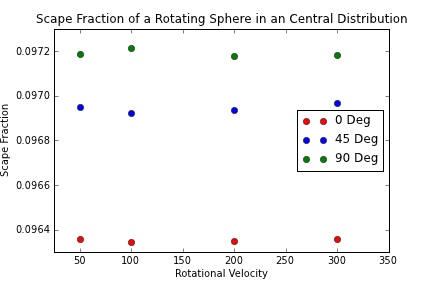
\includegraphics[width=0.45\textwidth]{FECentral5.png}
  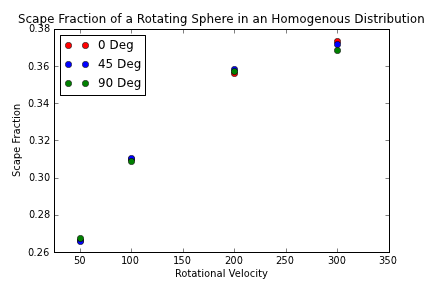
\includegraphics[width=0.45\textwidth]{FEHOM5.png}
  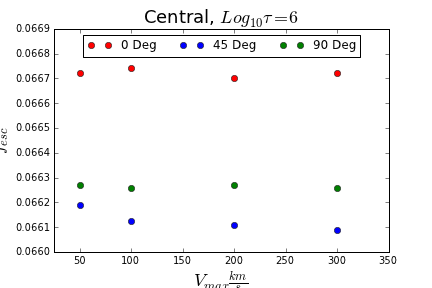
\includegraphics[width=0.45\textwidth]{FECentral6.png}
  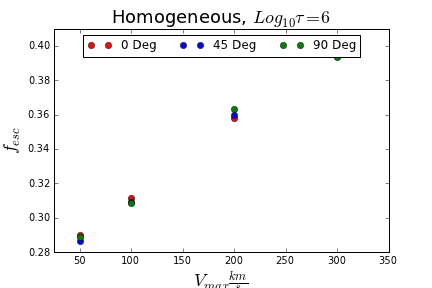
\includegraphics[width=0.45\textwidth]{FEHOM6.png}
  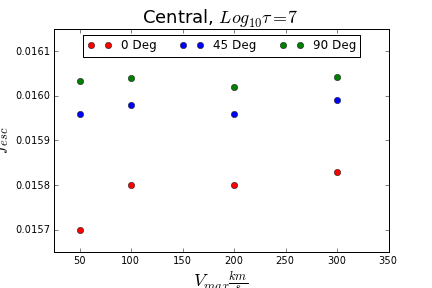
\includegraphics[width=0.45\textwidth]{FECentral7.png}
  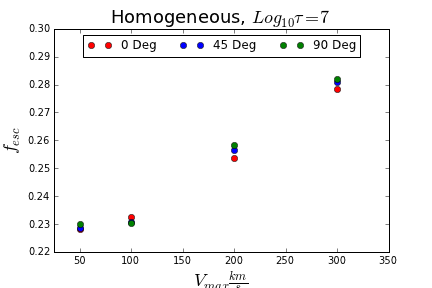
\includegraphics[width=0.45\textwidth]{FEHOM7.png}
  \label{figure:escape}\caption{Escape fraction for all the models. Left
    panels show the central distribution, while right panels show the
    homogeneous distribution} 
\end{figure*}

When the distribution is homogeneous the effect of velocity in the
escape fraction is clear while in the central model the effect is not
notorious. 
The main effect is that the escape fraction increase as the velocity
increase.  


\section{Discussion}
\label{sec:discussion}

\section{Observational implications}


\section{Conclusions}

\section*{Acknowledgements}

\section*{Appendix A: Tables}

\begin{table}
\begin{center}
\begin{tabular}{ccc}\hline          
Velocity (Km/s) & Maximum 1 position & Maximum 2 position \\ \hline
50 & -16.2695 & 16.23705 \\ 
100 & -15.66496 & 15.33504 \\ 
200 & -16.93149 & 14.56851 \\ 
300 & -13.40048 & 16.09952 \\ \hline 
\end{tabular} 
\caption{Optical Depth $\tau= 10^{7}$, Central Distribution}
\end{center}
\end{table}

\begin{table}
\begin{center}
\begin{tabular}{ccc}\hline 
Velocity (km/s) & Maximum 1 position & Maximum 2 position\\ \hline
50 & -7.46286 & 6.53714 \\ 
100 & -7.53357 & 6.96643 \\ 
200 & -8.17453 & 7.32547 \\ 
300 & -6.81487 & 6.18513 \\ \hline 
\end{tabular} 
\end{center}
\caption{Optical Depth $\tau = 10^{6}$, Central Distribution}
\end{table}

\begin{table}
\begin{center}
\begin{tabular}{ccc}\hline 
Velocity(Km/s) & Maximum 1 position & Maximum 2 position\\ \hline
50 & -4.33708 & 3.66292 \\ 
100 & -4.27326 & 3.72674 \\ 
200 & -3.7737 & 3.7263   \\ 
300 & -3.84903 & 4.15097 \\ \hline 
\end{tabular}
\caption{Optical Depth $\tau=10^{5}$, Central distribution} 
\end{center}
\end{table}

Line width\\

\begin{table}
\begin{center}
\begin{tabular}{ccc}\hline 
Velocity(Km/s) & FWHM & $\theta$\\ \hline 
50 & 12.62 & $0^{o}$ \\ 
50 & 12.72 & $45^{o}$ \\ 
50 & 12.93 & $90^{o}$ \\ 
100 & 14.07 & $0^{o}$ \\ 
100 & 14.48 & $45^{o}$ \\ 
100 & 15.00 & $90^{o}$ \\ 
200 & 16.90 & $0^{o}$  \\ 
200 & 18.51 & $45^{o}$ \\ 
200 & 21.24 & $90^{o}$ \\ 
300 & $24.69^{*}$ & $0^{o}$ \\ 
300 & $25.79^{*}$ & $45^{o}$  \\ 
300 & $27.73^{*}$ & $90^{o}$ \\ \hline
\end{tabular}
\caption{Lines Widhts for a Central Distribution and $\tau=10^{7}$} 
\end{center}
\end{table}


Escape fraction\\

\begin{table}[H]
\begin{center}
\begin{tabular}{ccccc}\hline 
Model & Velocity (km/s) & $\theta$ & Dust $\sum (s)$& $\sum (s)$\\ \hline 
Homogeneous & 50 & $0^{o}$& 13293.06 &49939.53\\ 
Homogeneous & 50 & $45^{o}$& 13291.04 &50001.59\\ 
Homogeneous & 50 & $90^{o}$ & 13348.76 &49922.73\\ 
Homogeneous & 100 & $0^{o}$ & 15527.69 &50114.11\\ 
Homogeneous & 100 & $45^{o}$ & 15511.56 &49967.17\\ 
Homogeneous & 100 & $90^{o}$ & 15401.71 & 49833.65\\ 
Homogeneous & 200 & $0^{o}$  & 17830.85 & 50078.69\\ 
Homogeneous & 200 & $45^{o}$ & 17932.87 & 50064.42\\ 
Homogeneous & 200 & $90^{o}$ & 17830.85  & 49931.748\\ 
Homogeneous & 300 & $ 0^{o}$ & 18687.33 & 50048.33 \\ 
Homogeneous & 300 & $45^{o}$ & 18572.12& 49922.67\\ 
Homogeneous & 300 & $90^{o}$ & 18421.79 & 49979.37\\ \hline
\end{tabular}
\caption{Escape fraction for a Homogeneous Distribution and optical depth $10^{5}$.} 
\end{center}
\end{table}


\begin{table}
\begin{center}
\begin{tabular}{ccccc} \hline 
Model & Velocity (km/s) & $\theta$ & Dust $\sum (s)$& $\sum (s)$ \\  \hline 
Central & 50 & $0^{o}$ & 4809.881 & 49917.069 \\ 
Central & 50 & $45^{o}$ & 4829.21 & 49811.79 \\ 
Central & 50 & $90^{o}$ & 4845.108 & 49853.039\\ 
Central & 100 & $0^{o}$ & 4809.665 & 49921.30 \\  
Central & 100 & $45^{o}$ & 4828.65 & 49820.13 \\ 
Central & 100 & $90^{o}$ & 4846.45 & 49854.0 \\ 
Central & 200 & $0^{o}$  & 4809.63 & 49917.64 \\ 
Central & 200 & $45^{o}$ & 4829.25 & 49818.49 \\ 
Central & 200 & $90^{o}$ & 4844.89 & 49856.66 \\ 
Central & 300 & $ 0^{o}$ & 4810.56 & 49922.98\\ 
Central & 300 & $45^{o}$ & 4831.16 & 49823.33\\ 
Central & 300 & $90^{o}$ & 4845.33 & 49858.48\\ \hline
\end{tabular}
\caption{Escape fraction for the central Distribution and optical depth $10^{5}$.} 
\end{center}
\end{table}


% Bibliography
%-----------------------------------------------------------------
%\begin{thebibliography}{99}

%\bibitem{Cd94} Author, \emph{Title}, Journal/Editor, (year)

%\end{thebibliography}

\end{document}
